\chapter{Problem statement and assessment}
\label{chap:probass}
\textit{\initial{T}his chapter detail the issues associated with the two questions described in the introduction and present its assessment. The plan of this chapter is as follows:
}
\minitoc

\newpage

The privileged domain, the dom0 in Xen, is a crucial element for a good yield of applications running inside virtual machines and for the \glspl{dc} management tasks using its resources. Here we detail the issues associated with the problematic in order to prove the relevance of this work. Let's recall the questions raised in the problematic : 

\begin{itemize}
    \item ($Q_1$) how should resources be allocated to the dom0? 
    \item ($Q_2$) how should these resources be organised in a \acrshort{numa} architecture ? 
\end{itemize}

\section{($Q_1$) Dom0 sizing}

The commonly used strategy is to statically allocate a fixed amount of resources to the dom0. A static resource allocation strategy consists in the allocation to the dom0, at server startup, of a given amount of resource which stays unchanged during its life time. Most data centers follow this strategy, including the research works that we studied \citep{livemigration,livemigration2,work01,work02,work03,work04}. For instance, we can observe such a static dom0 allocation policy in Amazon \acrshort{ec2} \citep{aws-ec2}, an allocated $c3$ $xlarge$ is supposed to receive $20$ processors, but only $16$ are available for virtual machine instances. Other processors are reserved for the dom0. 

\paragraph{}
\begin{bidentidad2}
\centering \textbf{There isn't any defined method to estimate the amount of resources which is required for the dom0 to perform correctly}. 
\end{bidentidad2}

This allocation is totally arbitrary. Server virtualization systems providers do not provide any recommendation regarding this issue. The only recommendation that we found for the dom0 resource allocation comes from \textbf{Oracle} \citep{oracle}, which proposes a dom0 memory allocation based on the rule given by the following rule. \textbf{E stands for whole part.}

\begin{equation*}
    \mathbf{dom0\_mem = 502 + E(physical\_mem\times 0.0205)}
\end{equation*}

\par The problem with such a static allocation is that the amount of resources required by the dom0 is not constant, as it depends on the \textbf{dom0 workload}. The tasks executed by the dom0 can be organized into two groups: 

\begin{itemize}
    \item those that do not depend on the domUs (these tasks are related to the to the management of the \glspl{dc}) and 
    \item those that depend on the domUs (most of these tasks are involved when the domUs are requesting device drivers).
\end{itemize}

The amount of resources required by tasks from the second group is \textbf{variable} as it depends on the activity of the domUs. To demonstrate it, we carried out an experiment (whose experimental setup is shown on Figure \ref{fig:expe-setup1}) consisting of measuring the variation of the dom0 \acrshort{cpu} load according to a number of domU executing an \textbf{IOZONE} \citep{iozone} benchmark.

\begin{figure}[!h]
    \centering
    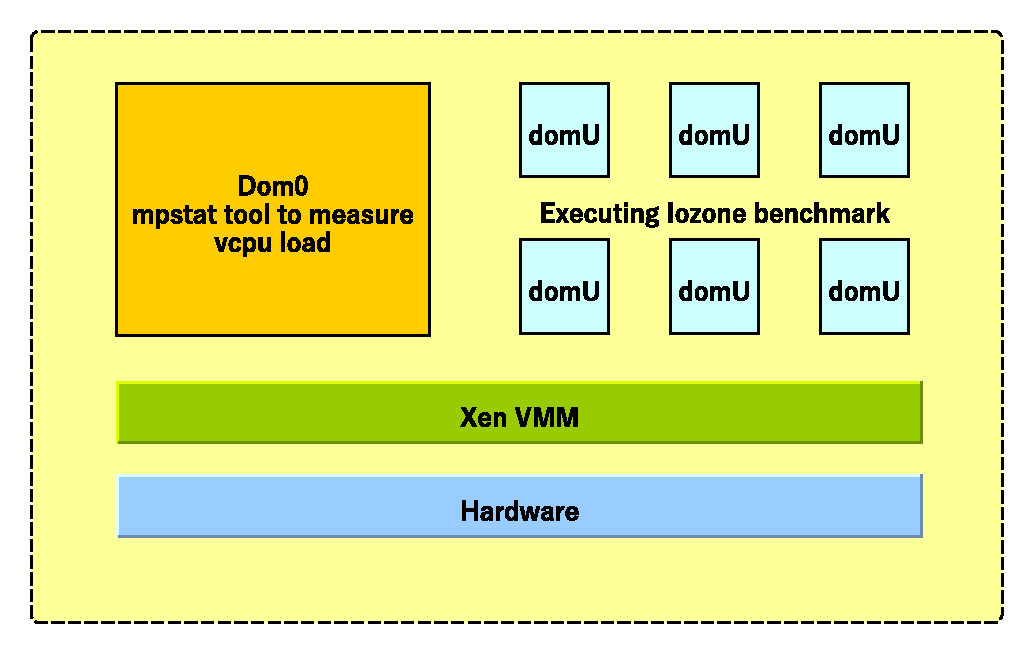
\includegraphics[scale=0.65]{fig03/expe1.pdf}
    \caption{Experimental setup to show the variation of resources required by the tasks from the second group.}
    \label{fig:expe-setup1}
\end{figure}

As shown on Figure \ref{fig:expe1}, we observe that the dom0's load heavily depends on the domU. The consequence is that a static allocation can lead to two situations: either \textbf{the dom0 lacks resources}, or \textbf{the resources are overbooked by the dom0.} These two situations can be harmful both for the cloud provider and for the user's applications.

\subsection{Consequences of an undersized dom0}
A lack of resource in the dom0 can have significant impacts both for applications executed in the domUs and for administrative services executed in the dom0. 

\paragraph{Impact on user's applications.} To prove it, we conducted an experiment (whose setup is shown on figure \ref{fig:expe2}), where we varied the number of co-located domU guests which executes \acrshort{io} intensive workloads with a domU guest executing a Wordpress application. The dom0 was allocated two processors while each domU was allocated one processor. In order to prevent any contention (e.g \acrshort{qpi} link contention), all processors (from dom0 or domUs) were allocated on the same socket. The low-level cache is not a limiting factor for \acrshort{io} intensive applications \citep{work03}.  

\begin{figure}[!h]
    \centering
    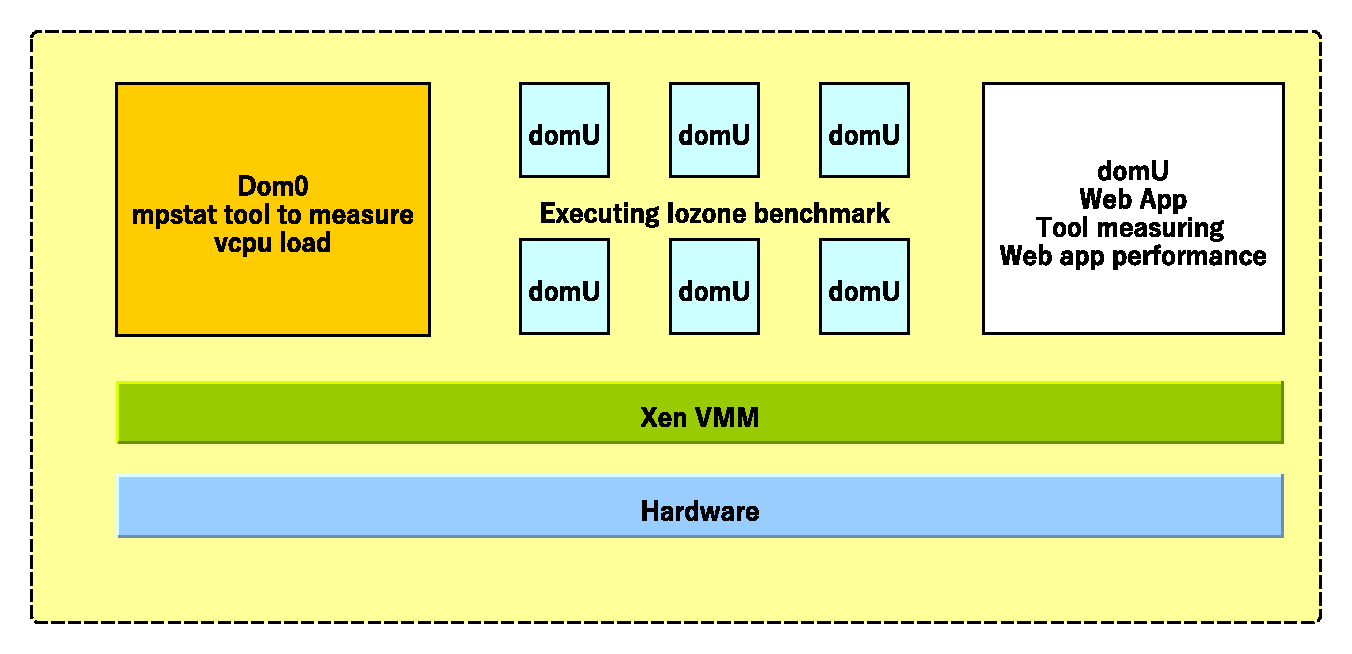
\includegraphics[scale=0.65]{fig03/expe2.pdf}
    \caption{Experimental setup to show the impact of dom0's resources on user's application.}
    \label{fig:expe2}
\end{figure}

Figure \ref{fig:expe21} presents the dom0 \acrshort{cpu} load and the domU web application performance. The first observation is that the dom0 load varies according to the \acrshort{io} activity of Domus. This variation is explained by the fact the dom0 embeds the back-end (from the split driver) and the driver is responsible for accessing the hardware. The second observation is that the web application performance decreases when the dom0 lacks \acrshort{cpu} resources since \acrshort{cpu} resources are statically allocated to the dom0. Therefore, \textbf{performance predictability} is compromised, which is one of the main issues in cloud computing environments \citep{predictability,predictability1,predictability2,predictability3,predictability4}.

\paragraph{Impact on virtual machine management tasks.} The dom0 hosts the execution of virtual machine administration commands, the most important commands being: \textbf{create, destruction, migration} of virtual machines and modification of resources allocated to the virtual machines. The limitation of dom0 allocated resources leads to a variation of the execution time of these commands since they require a significant amount of resources. For instance, virtual machine migration requires a lot of \acrshort{cpu} to detect dirty pages from the virtual machine being migration \citep{livemigration,livemigration2}. We conducted an experiment (whose setup is shown on Figure \ref{fig:expe3}) to show the impact of dom0's resources on these tasks. On Figure \ref{fig:expe11} and \ref{fig:expe23}, we observe that the dom0 load has a significant impact on these execution times, and may dramatically influence higher level services such as auto-scaling (which relies on virtual machine creations and destructions) or consolidation (which relies on virtual machine migrations). 

\begin{figure}[!h]
    \centering
    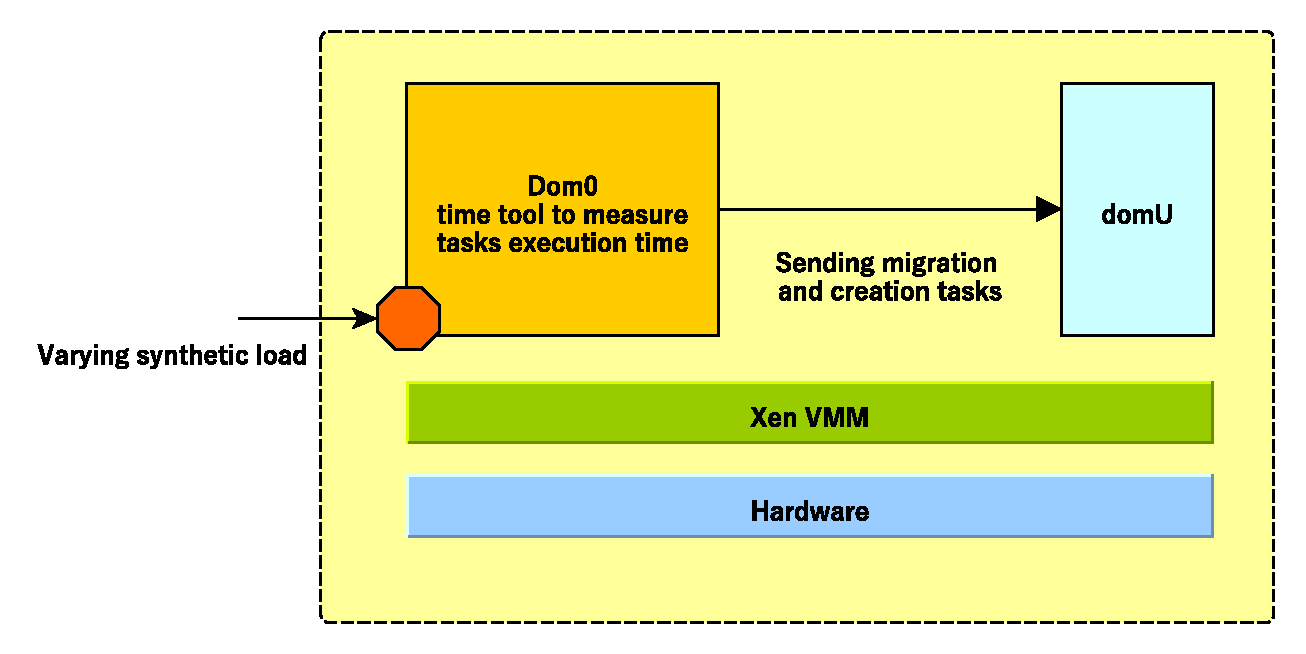
\includegraphics[scale=0.65]{fig03/expe3.pdf}
    \caption{Experimental setup to show the impact of dom0's resources on management tasks.}
    \label{fig:expe3}
\end{figure}

\paragraph{Impact on \glspl{dc} management services.} An overload of the dom0 (due to an overload of hosted virtual machines, which may be a consequence of a \textbf{denial service attack}) can significantly impact the management system of a \glspl{dc}. If we consider an \textbf{OpenStack} system, each server executes (in its dom0) a set of tasks which enable its management in the \glspl{dc}. If these tasks are no longer reachable from the central controller (Nova), the server is considered out of order, which may trigger a recovery procedure. We experimented with such a situation in a small OpenStack cluster composed of one compute node and one controller node (as shown on figure \ref{fig:expe4}. OpenStack components were configured with default values (a timeout of 300s). We allocated to the dom0 of the compute node two vCPUs and created several domUs on this node. Then, we executed in these virtual machines the Iozone benchmark in order to overload the dom0. We observed that when reaching a given load ($75\%$) in the dom0, the controller considered that the compute node was failing.

\begin{figure}[!h]
\centering
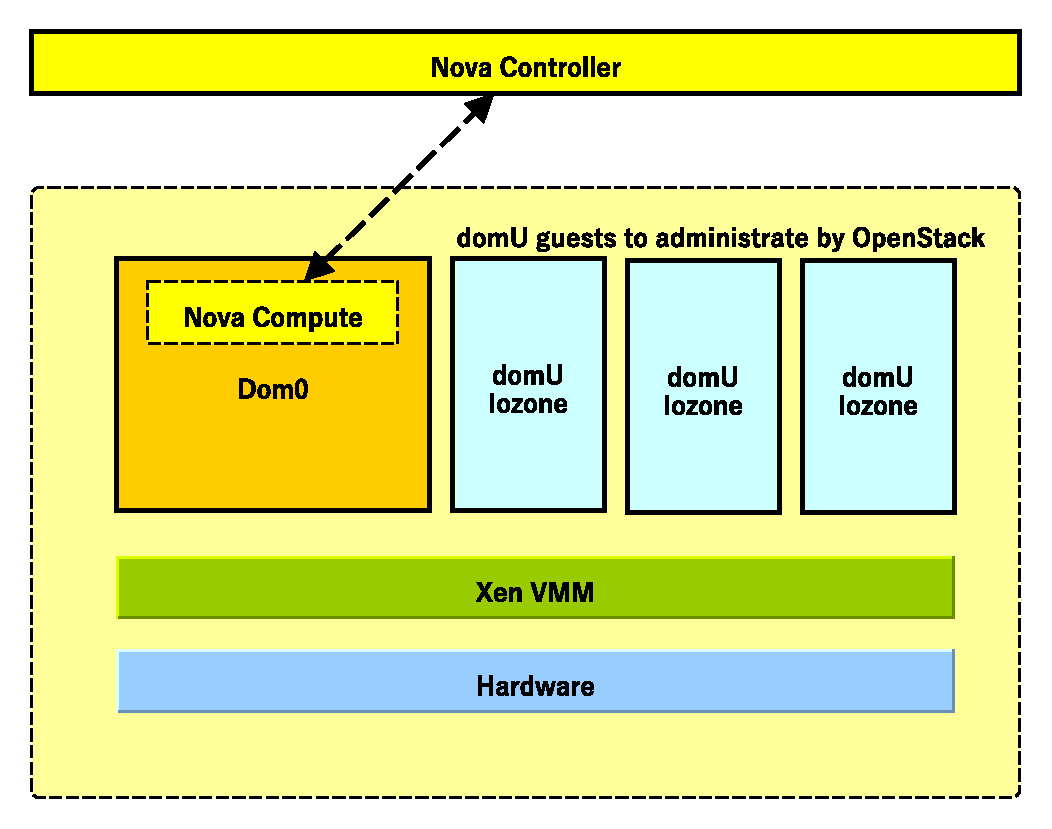
\includegraphics[scale=0.65]{fig03/expe4.pdf}
\caption{Experimental setup to show the impact of dom0's resources on the data center management services.}
\label{fig:expe4}
\end{figure}

\subsection{Consequence of an oversized dom0}
Overprovisioning is a source of resource waste as shown by many works. Most previous works studied domU overprovisioning and its associated waste \citep{predictability,predictability1,predictability4}. We are here interested in dom0 over-provisioning. In order to evaluate it, we relied on \textbf{Google traces}, considering that container workloads were executed in Domus. We statically allocated to the dom0 one socket from a machine. Assuming that domUs are executing \textbf{Hadoop} tasks, we experimentally determined the relationship between resources consumed by an Hadoop task and resources consumed by the dom0. Then, we evaluated on a period of traces (29 days) the amount of unused (wasted) resources in the dom0. These resources could have been used to host additional domUs or to increase the consolidation ratio. If we consider the smallest task in Google's \glspl{dc}, wasted resources could have satisfied 1440 tasks.

\section{($Q_2$) Dom0 location and Review}
The location of resources allocated to the dom0 may significantly influence virtual machine's application performance.


\paragraph{Performance of \acrshort{io} intensive applications.} We performed an experiment (in a \acrshort{numa} architecture as shown on Figure \ref{fig:expe6}) to demonstrate the influence of dom0 resources location on the performance of \acrshort{io} intensive applications. We executed a web application in a virtual machine whose \acrshort{cpu} and memory resources are located on one socket. Then, we varied the location of the resources (\acrshort{cpu} and memory) allocated to the dom0. Figure \ref{fig:expe26} presents the performance of the web application in different situations. We observe that the best performance is obtained when resources from the virtual machine and the dom0 are co-located on the same socket (socket 8). Indeed, co-location prevents \textbf{remote memory accesses} between sockets in the NUMA architecture.

\begin{figure}[!h]
\centering
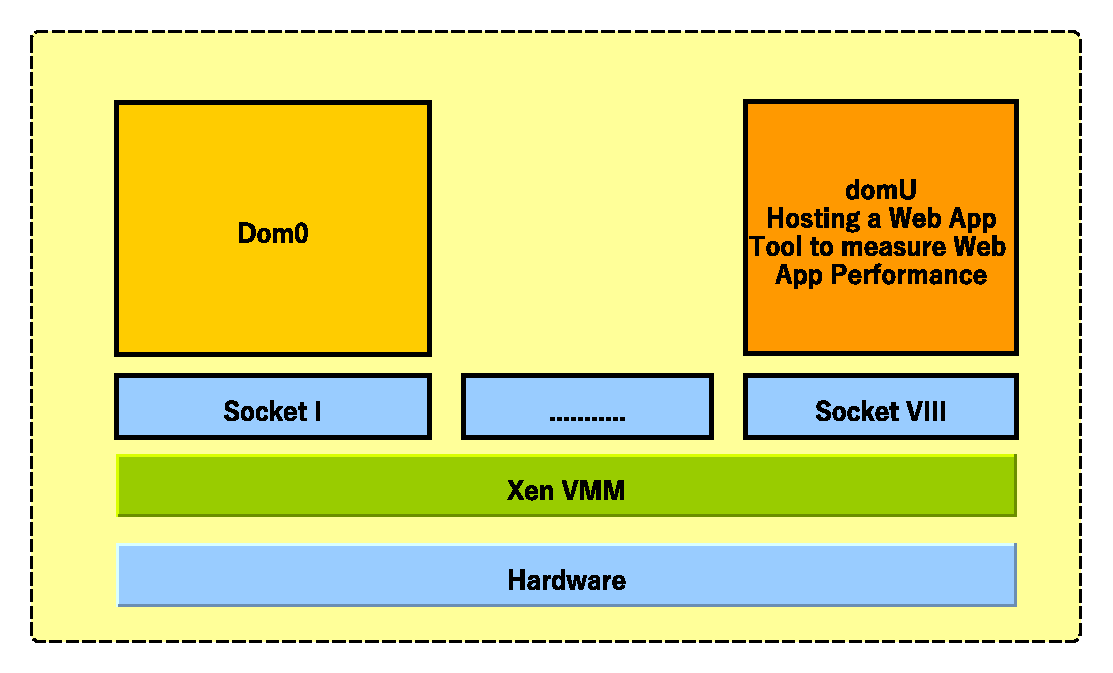
\includegraphics[scale=0.65]{fig03/expe6.pdf}
\caption{Experimental setup to show the impact of dom0's resources location on domU IO applications.}
\label{fig:expe6}
\end{figure}

\paragraph{Virtual machine migration.} Figure \ref{fig:expe25} presents the virtual machine migration time according to the location of the dom0 \acrshort{vcpu}s on the machine's sockets (as shown on figure \ref{fig:expe5}. When the dom0 \acrshort{vcpu}s are co-located with the virtual machine to migrate (on socket 8), migration is much faster since remote memory accesses between sockets are avoided. We observed the same behavior for the removal of a virtual machine (since the scrub operation is faster when memory is accessed locally), which has a strong impact on the autoscaling mechanism \citep{work03}.


\begin{figure}[!h]
\centering
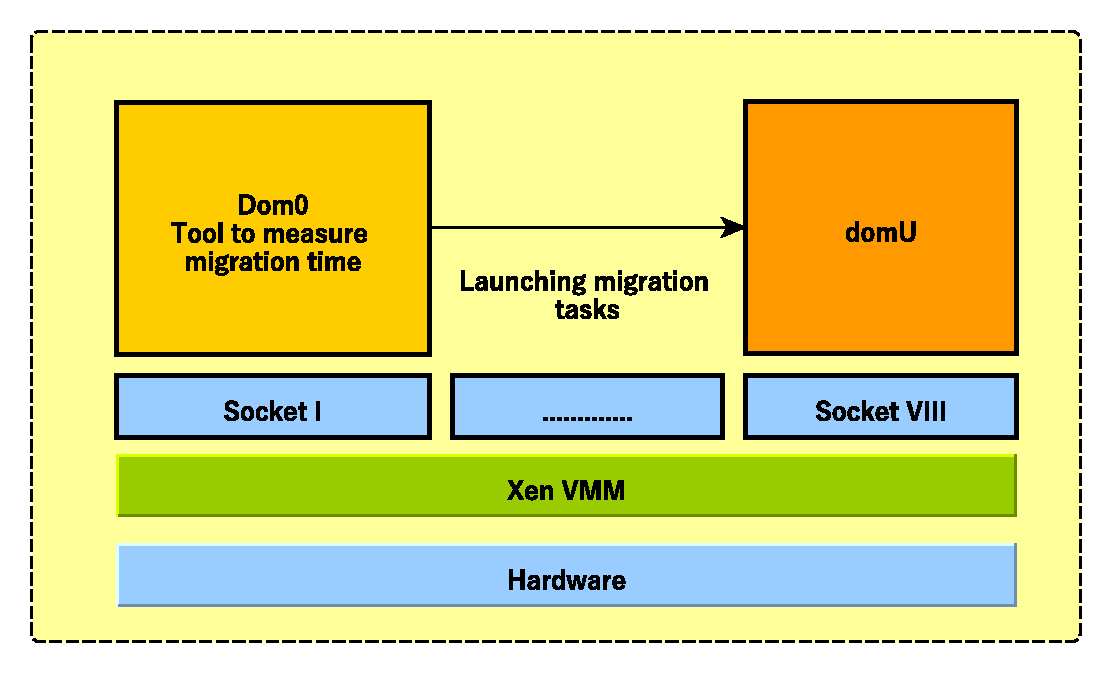
\includegraphics[scale=0.60]{fig03/expe5.pdf}
\caption{Experimental setup to show the impact of dom0's resources location on domU migration.}
\label{fig:expe5}
\end{figure}

\begin{figure}[!h]
\begin{minipage}[b]{.5\linewidth}

\centering
\begin{tikzpicture}
\begin{axis}[legend style={at={(0.5,-0.1)},anchor=north},
title=Dom0's load variation,
legend entries = {Load on dom0 (\%)}
]
\addplot table {chapters/chapter03/data/expe1.dat};

\end{axis}
\end{tikzpicture}
\subcaption{{\small Dom0's load against the number of domU \\ guests executing the Iozone benchmark.}}
\label{fig:expe1}
\end{minipage}
%%%%%%%%%%%%%%%%%%%%%%%%
\hfill 
\begin{minipage}[b]{.5\linewidth}
\centering
\begin{tikzpicture}
\begin{axis}[legend style={at={(0.5,-0.1)},anchor=north},
title = DomU migration time,
legend entries = {Migration time (s)}]
\addplot table {chapters/chapter03/data/expe23.dat};
\end{axis}
\end{tikzpicture}
\subcaption{{\small DomU migration time against the load on the dom0's \acrshort{vcpu}}.}
\label{fig:expe23}
\end{minipage}
\caption{Experimental results, first group}

\end{figure}
%%%%%%%%%%%%%%%%%%%%%%%%%%%%%%%%%%%%%%%%%%%%%%%%%%
%\vspace{-5cm}
\begin{figure}[!h]\small
\begin{minipage}[b]{.5\linewidth}
\centering
\begin{tikzpicture}
\begin{axis}[legend  style={at={(0.5,-0.1)},anchor=north},
title=Dom0's load and domU web app Performance,
xlabel={Number of domU guest},
legend entries = {Web App performance (\%), Load on dom0 (\%)}
]
\addplot table {chapters/chapter03/data/expe21.dat};
\addplot table {chapters/chapter03/data/expe22.dat};

\end{axis}
\end{tikzpicture}
\subcaption{{\small Dom0's load and domU web application yield.}}
\label{fig:expe21}
\end{minipage}
\hfill 
%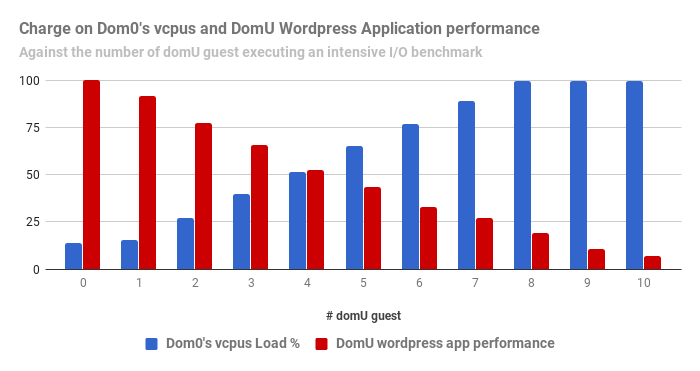
\includegraphics[width=\linewidth]{fig03/chart_result_2.png}
%%%%%%%%%%%%%%%%%%%
\begin{minipage}[b]{.5\linewidth}
\centering
\begin{tikzpicture}
\begin{axis}[legend style={at={(0.5,-0.1)},anchor=north},
title=DomU creation task time,
legend entries = {\#domU=1 (ms), \#domU=5 (ms)}
]
\addplot table {chapters/chapter03/data/expe24.dat};
\addplot table {chapters/chapter03/data/expe241.dat};


\end{axis}
\end{tikzpicture}
\subcaption{{\small DomU creation task time against the dom0's load}}
\label{fig:expe11}
\end{minipage}
\caption{Experimental results, second group}

\end{figure}


\section{Review}
From all the experiments we conducted, it is clear that a non-intelligent allocation for the dom0 will lead to adverse consequences for the provider and its customers. We identified the main problem and in the next chapter, we present our approach to this problem.



\begin{figure}[!h]
\begin{minipage}[b]{.5\linewidth}

\centering
\begin{tikzpicture}
\begin{axis}[legend style={at={(0.5,-0.1)},anchor=north},
title={DomU migration time},
legend entries = {domU migration time (s)}
]
\addplot table {chapters/chapter03/data/expe25.dat};

\end{axis}
\end{tikzpicture}
\subcaption{{\small DomU migration time against the socket}.} \label{fig:expe25}
\end{minipage}
%%%%%%%%%%%%%%%%%%%%%%%%
\hfill 
\begin{minipage}[b]{.5\linewidth}
\centering
\begin{tikzpicture}
\begin{axis}[legend style={at={(0.5,-0.1)},anchor=north},
title = {DomU web application yield},
legend entries = {Throughput (\acrshort{mb}/s)}]
\addplot table {chapters/chapter03/data/expe26.dat};
\end{axis}
\end{tikzpicture}
\subcaption{{\small DomU web application yield against the socket.}}
\label{fig:expe26}
\end{minipage}

\caption{Experimental results, third group}
\end{figure}

%\newpage 
%\section{Observations}
%\newpage \newpage \newpage \newpage \newpage
%\paragraph{\Large{Review.}}


